\documentclass[12pt, a4paper, oneside]{ctexart}
\usepackage{amsmath, amsthm, amssymb, bm, color, framed, graphicx, hyperref, mathrsfs, float}
\pagestyle{plain}

% multi-column
\usepackage{tasks}
% itemize
\NewTasksEnvironment[label=(\arabic*), label-width=3ex]{exercise}

\everymath{\displaystyle}

\title{\textbf{第二次作业}}
\author{U08M11002 Fall 2023}
\linespread{1}
\definecolor{shadecolor}{RGB}{241, 241, 255}

\newcounter{problemname}
\newenvironment{problem}{\stepcounter{problemname}\par\noindent\textbf{题目\arabic{problemname}. }}{\\\par}
\newenvironment{warning}{\begin{shaded}\par\noindent\textbf{提交作业方式:}}{\end{shaded}\par}

\begin{document}

\maketitle

\hspace{1em}

\begin{problem}
$a,b \in \mathbb{R}, a \neq 0$,证明:
$$  \int_{-\infty}^{\infty} f(t) \delta(at-b) dt = \frac{1}{|a|} f(\frac{b}{a}) $$
\quad
\end{problem}

\begin{problem}
证明  $\int_{-\infty}^{\infty} f(t) \delta(t-t_0) dt = f(t_0)$.
\quad
\end{problem}

\begin{problem}
证明  $\int_{-\infty}^{\infty} f(t) \delta'(t) dt = -f'(0)$.
\quad
\end{problem}

\begin{problem}
证明:微分、积分(变上限积分)和延时器($y(t) = f(t-t_0)$)都是线性系统。
\quad
\end{problem}

\begin{problem}
证明以下系统\textbf{不是}时不变系统(LTI):
\begin{exercise}(2)
	\task (变系数)$y=tf(t)$
	\task (反转)$y=f(-t)$
	\task (伸缩)$y=f(\alpha t)$
\end{exercise}
\quad
\end{problem}

\begin{problem}
判断下列系统的因果性:
\begin{exercise}(2)
	\task $y(t) = f(t-2)$
	\task $y(t) = f(t+2)$
\end{exercise}
\quad
\end{problem}

\begin{problem}
判断下列系统是否为线性的、时不变的、因果的。假设系统均为零状态系统 。
\begin{exercise}(2)
	\task $y(t) = \frac{d^2}{d^2t} f(t)$
	\task $y(t) = f(t) U(t)$
	\task $y(t) = \sin[f(t)] U(t)$
	\task $y(t) = f(1-t)$
	\task $y(t) = f(2t) $
	\task $y(t) = f^2(t) $
	\task $y(t) = \int_{-\infty}^{t} f(\tau) d\tau $
	\task $y(t) = \int_{-\infty}^{5t} f(\tau) d\tau $
\end{exercise}
\quad
\end{problem}

\begin{problem}
线性时不变系统,当激励$f_1(t) = U(t)$ 时,响应 $y_1(t) = e^{-at} U(t)$。试求当激励$f_2(t) = \delta(t)$ 时,响应 $y_2(t)$的表达式。(假定起始时刻系统无储能。)
\quad
\end{problem}

\begin{problem}
	$f_1(t) = 3e^{-2t}U(t)$, $f_2(t) = 2U(t)$, $f_3(t) = 2U(t-2)$,求
	\begin{exercise}(2)
		\task $f_1(t) * f_2(t) $
		\task $f_1(t) * f_3(t) $
	\end{exercise}
	\quad
\end{problem}

\begin{problem}
	求下图中 $f_1(t)$ 和 $f_2(t)$ 的卷积。
	\begin{figure}[H]
		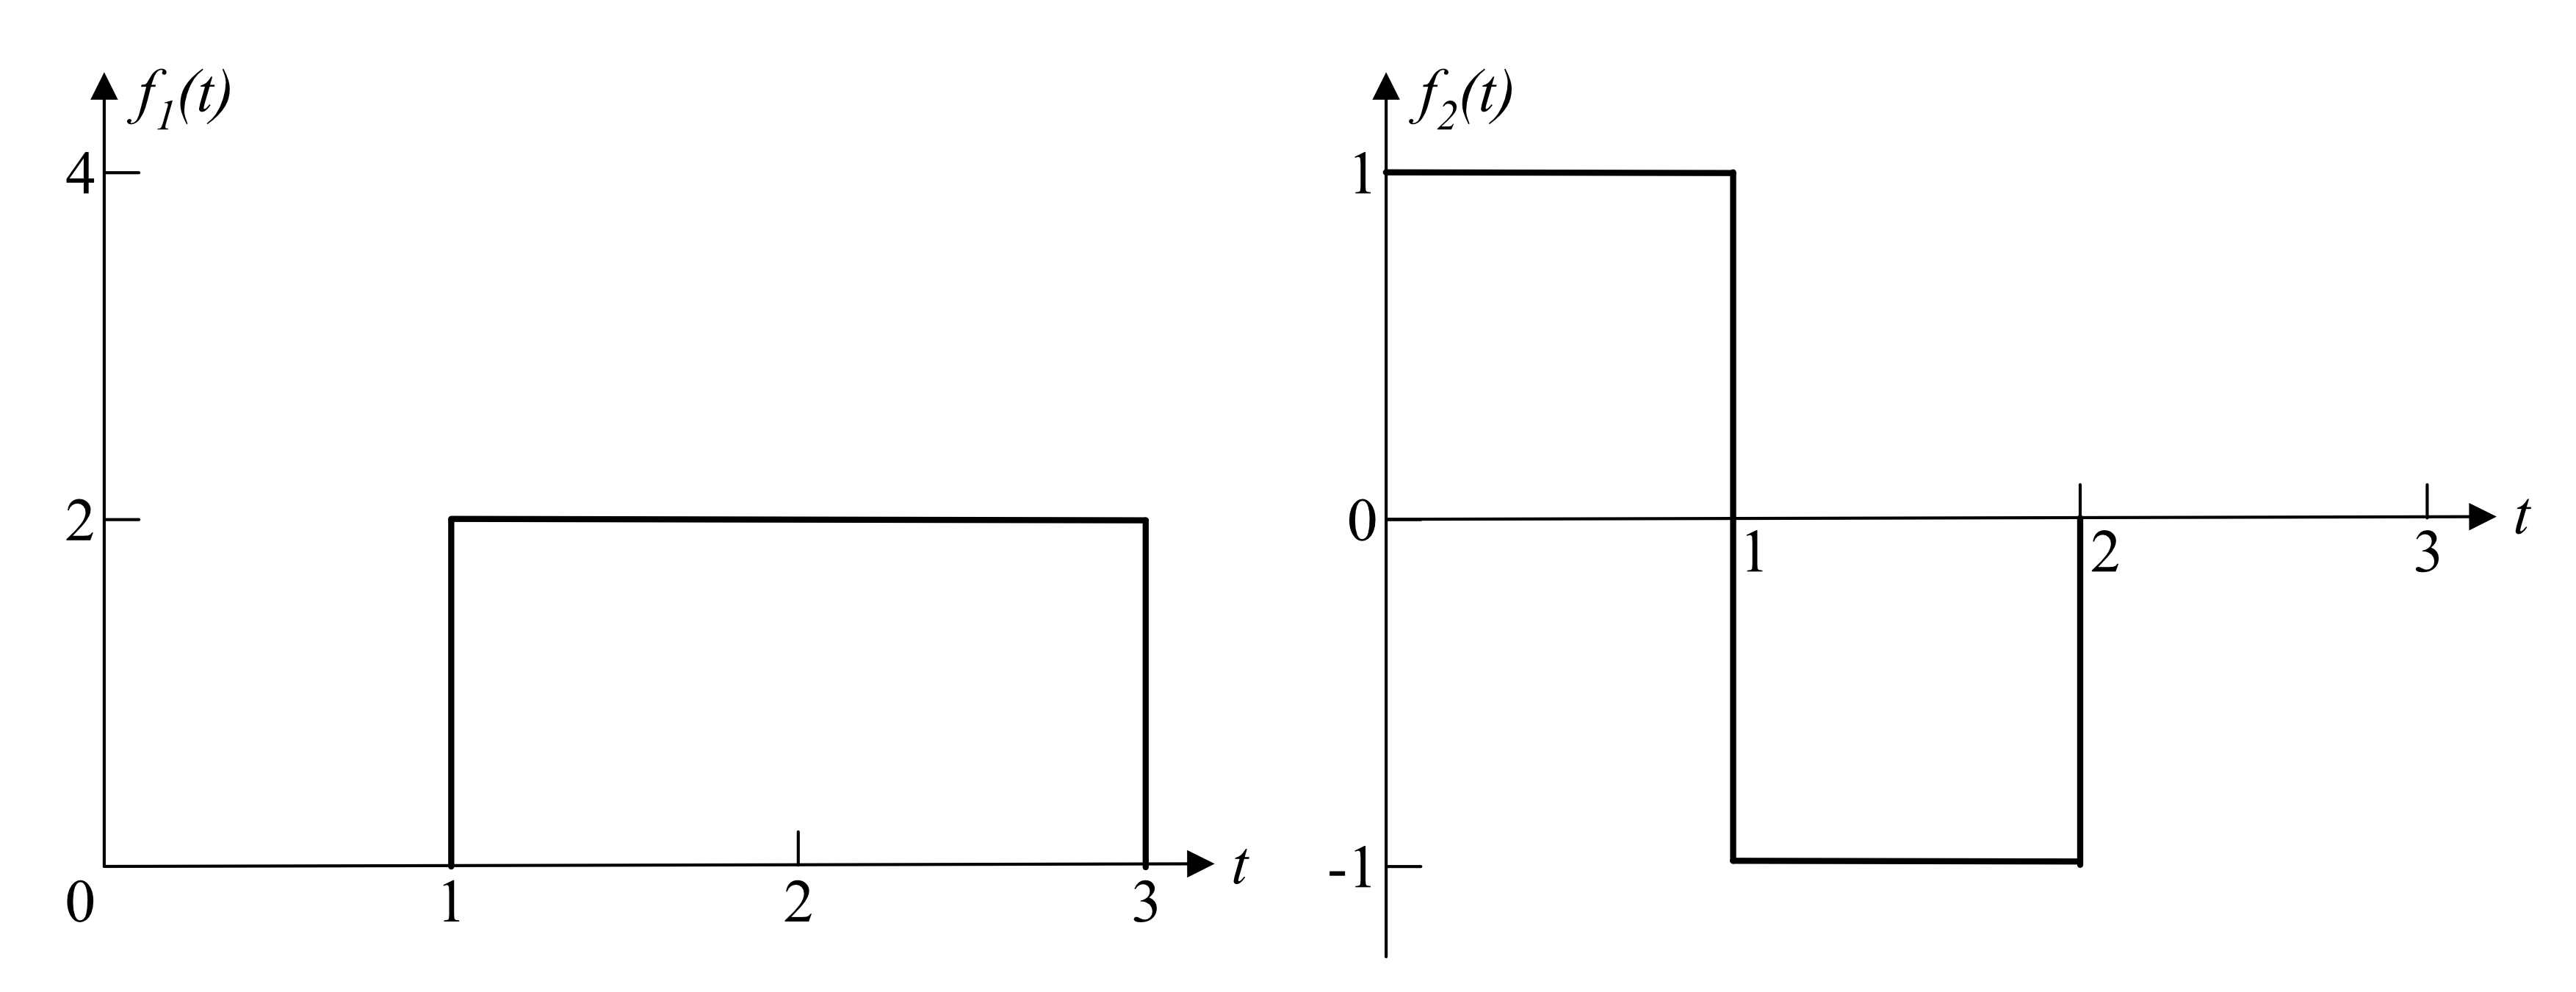
\includegraphics[width=12cm]{assets/hw3img1.png}
		\centering
	\end{figure}
	\quad
\end{problem}

\end{document}